\begin{frame}
    \begin{enumerate}
        \item Provider Model und Agent
        \item Tool calling (Langchain Tools) (MCP) (human interaction hook) (cli) (draw io) (send-mail)
        \item 1. Single Agent interactive unstructured output
        \item 2. Single Agent Reconnaissance unstructured output
        \item 3. POC Blueteam intrusion detection - not followed time and scope - unstructured output
        \item 4. Single Agent reconnaissance structure output (context-window, grammar -> why structured output create larger grammar)
        \item 5. Multi Agent reconnaissance structured output (issue with smaller models) () Containerlab evalutation smaller model
        \item 6. Multi Agent reconnaissance unstructured output
    \end{enumerate}
\end{frame}

\begin{frame}{Concept 1: Taming the Context}
    \framesubtitle{From one overloaded agent to a focused pipeline}

    \begin{columns}[T,onlytextwidth]
        \begin{column}{0.5\textwidth}
            \onslide<1-> {
                \textbf{\faExclamationTriangle~~The problem}
                \begin{itemize}
                    \item \scriptsize One agent does everything in a single long conversation
                    \item \scriptsize Every scan output piles up $\rightarrow$ the \textbf{context keeps growing}
                    \item \scriptsize Smaller models lose the thread and start failing
                    \item \scriptsize Cost and runtime become hard to predict
                \end{itemize}
            }
        \end{column}

        \begin{column}{0.5\textwidth}
            \onslide<2->{
                \textbf{\faProjectDiagram~~Our solution}
                \begin{itemize}
                    \item \scriptsize Split the task into \textbf{discovery $\rightarrow$ enumeration $\rightarrow$ assessment}
                    \item \scriptsize Each phase is a \textbf{fresh agent} with its own, small context
                    \item \scriptsize We pass on only the \textbf{distilled result}, not the whole history
                \end{itemize}
            }
        \end{column}
    \end{columns}

    \onslide<3->{
        \vspace{1.2em}
        \footnotesize \faInfoCircle~~Trade-off: Improves results when the context window is almost full, but adds orchestration overhead.
    }
\end{frame}


\begin{frame}{Concept 2: Keeping the Operator in Control}
    \framesubtitle{The agent proposes -- the human decides on risky actions}

    Merge with previous slide
    \begin{columns}[T,onlytextwidth]
        \begin{column}{0.5\textwidth}
            \textbf{\faExclamationTriangle~~The problem}
            \begin{itemize}
                \item \scriptsize An autonomous agent can run \textbf{any} command or send reports on its own
                \item \scriptsize In a security context that is unacceptable without oversight
            \end{itemize}
        \end{column}

        \begin{column}{0.5\textwidth}
            \onslide<3->{
                \textbf{\faHandPaper~~Our solution}
                \begin{itemize}
                    \item \scriptsize The agent \textbf{pauses} before sensitive actions and asks for a decision
                    \item[\faTerminal] \scriptsize Shell commands $\rightarrow$ \textbf{approve} before they run
                    \item[\faEnvelope] \scriptsize Sending a report $\rightarrow$ \textbf{approve / reject}
                    \item[\faComments] \scriptsize Open questions $\rightarrow$ operator \textbf{responds} in free text
                \end{itemize}
            }
        \end{column}
    \end{columns}

    \onslide<4->{
        \vspace{0.4em}
        \footnotesize \faRedo~~After the decision the agent resumes exactly where it stopped -- no restart, no lost progress.
    }
\end{frame}

\begin{frame}
    Merge with previous slide
    \begin{columns}
        \begin{column}{0.5\textwidth}
            \uncover<1-> {
                \textbf{Single Agent}
                \begin{itemize}
                    \item \scriptsize One prompt to achieve the goal
                    \item \scriptsize Long chain of tool calls, \textbf{growing context}
                    \item \scriptsize Smaller models fail as context fills up
                \end{itemize}
            }

            \vspace{0.6em}
            \uncover<2-> {
                \textbf{Multi Agent} \textit{\scriptsize divide-and-conquer}
                \begin{itemize}
                    \item \scriptsize Prompt split into steps; result fed into next agent
                    \item \scriptsize Smaller, focused context per step
                    \item \scriptsize Helps small models; may add overhead for frontier
                \end{itemize}
            }
        \end{column}

        \begin{column}{0.5\textwidth}
            \uncover<3-> {
                \begin{block}{Structured vs.\ Unstructured output}
                    \scriptsize
                    \textbf{Structured} (schema-constrained): great for automated metrics,
                    but \textbf{high failure rate} -- especially for small models.
                    \vspace{0.3em}\\
                    \textbf{Unstructured}: needed in the BFH lab where all models failed to
                    produce valid structured output; freed the agent but required manual evaluation.
                \end{block}
            }
        \end{column}
    \end{columns}
\end{frame}


\begin{frame}{Multi-Agent Reconnaissance Pipeline}
    \framesubtitle{Discovery $\rightarrow$ enumeration $\rightarrow$ assessment, each a fresh agent}

    \begin{figure}
        \centering
        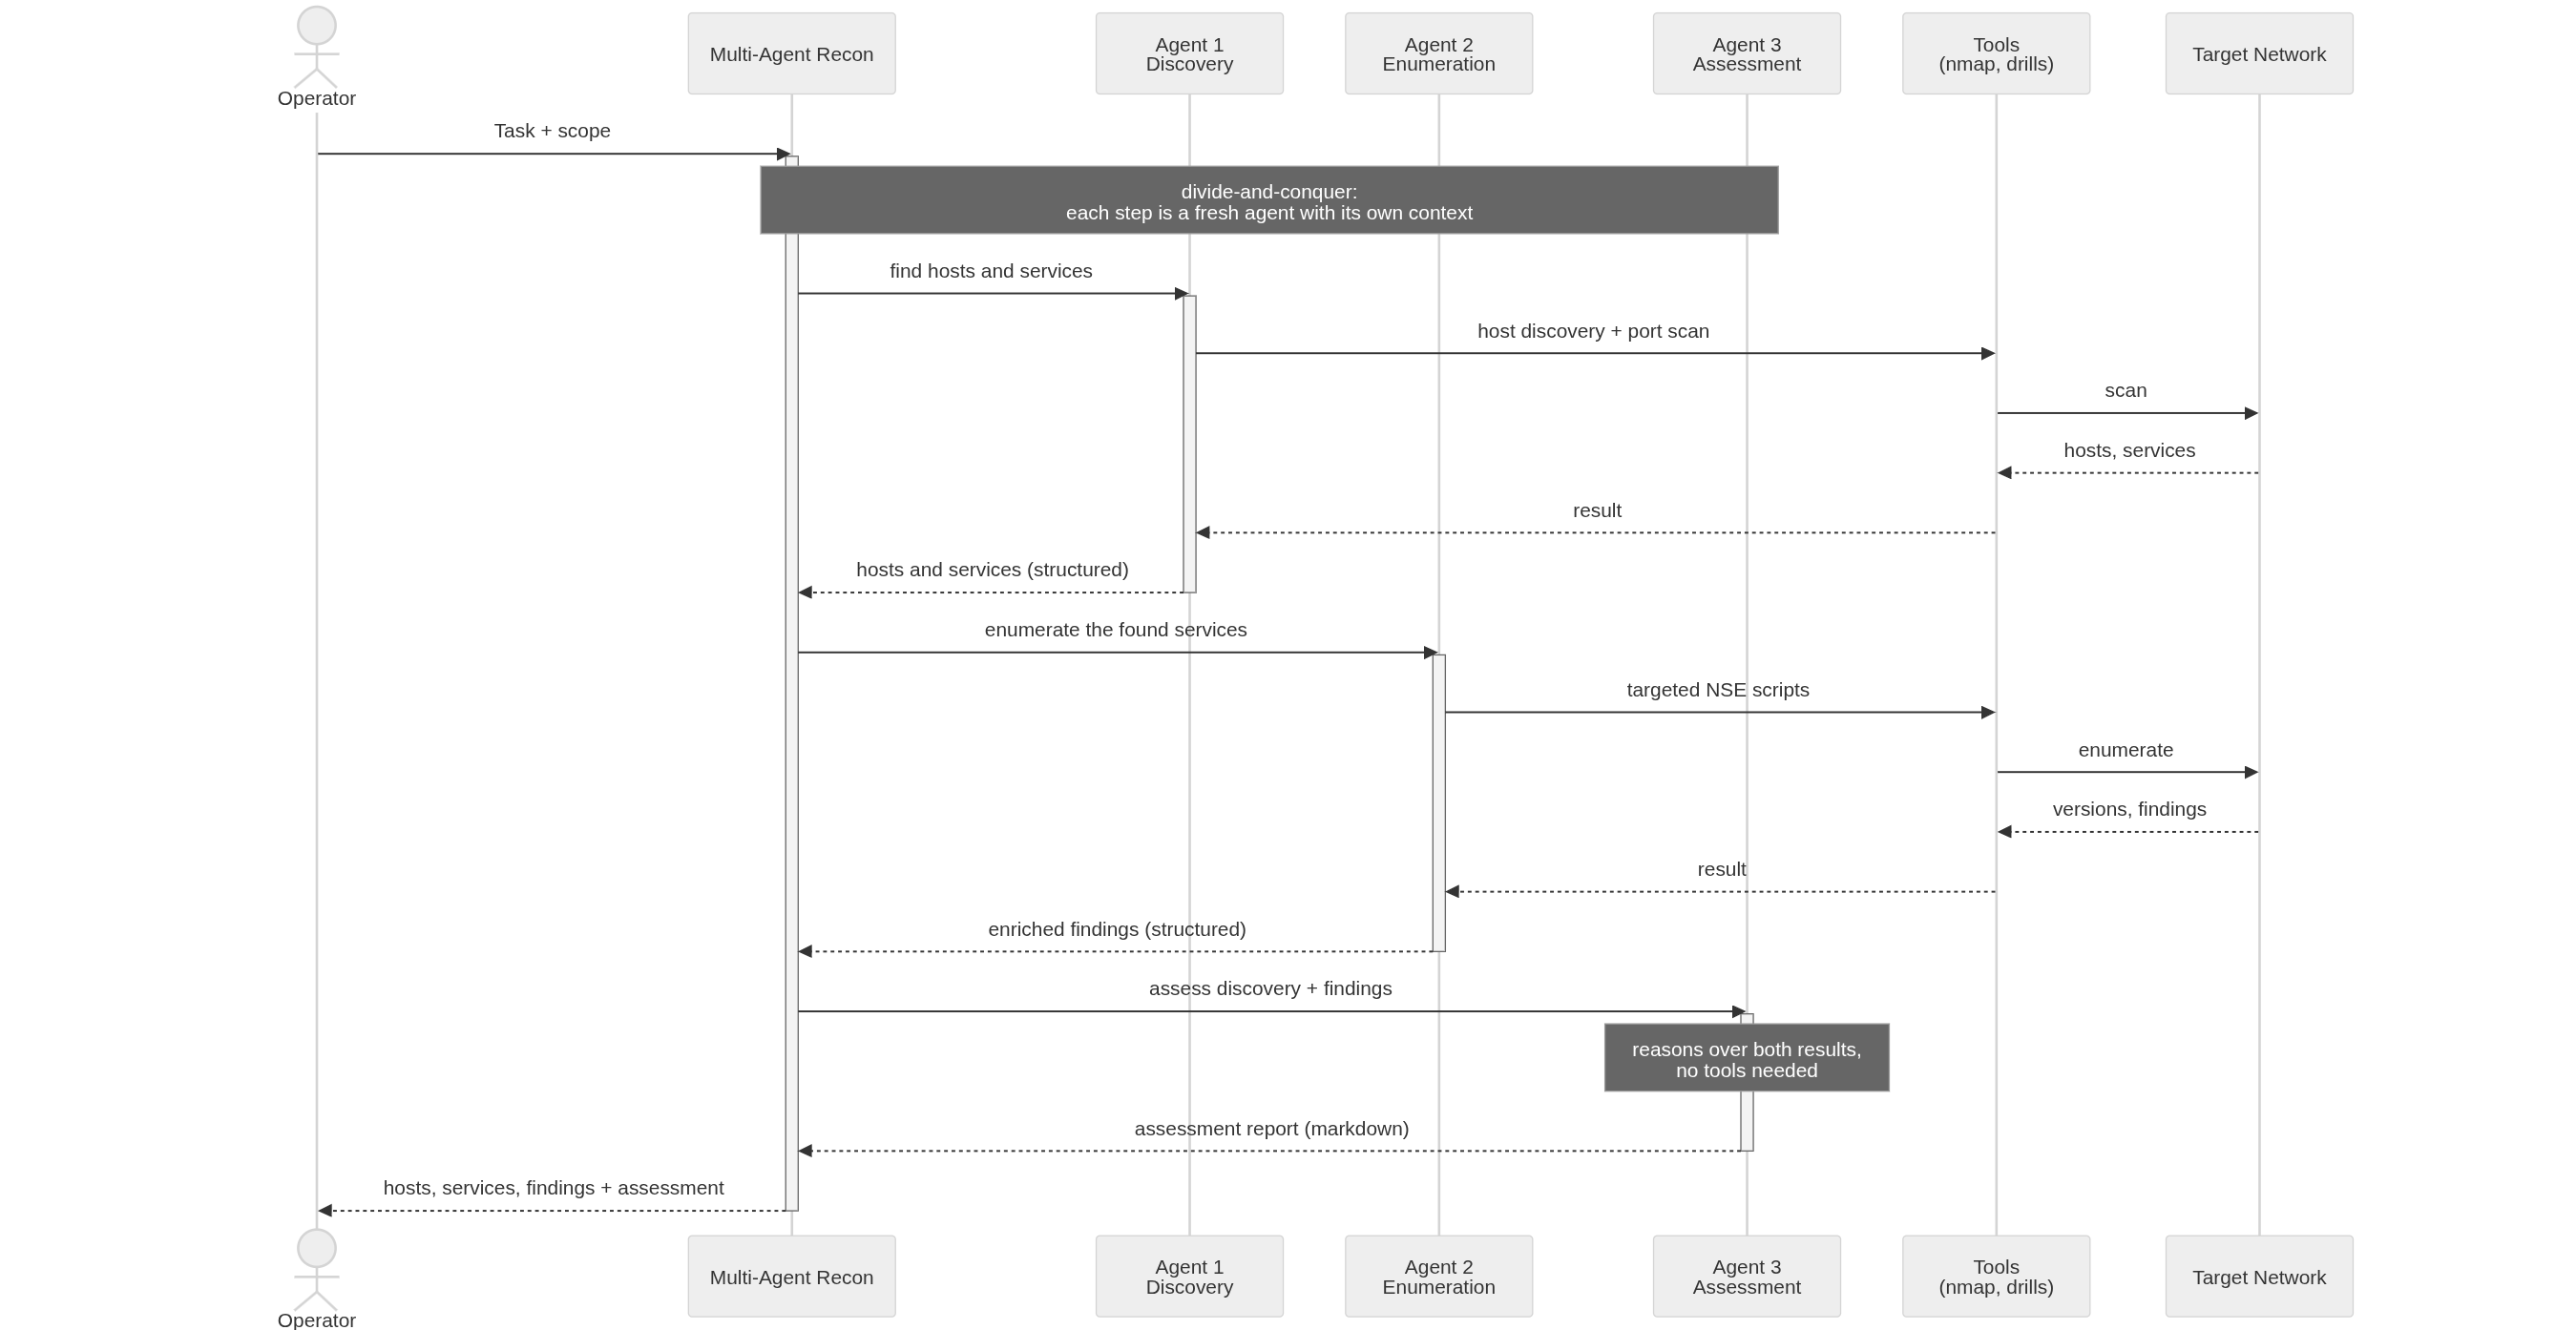
\includegraphics[width=\linewidth,height=0.78\textheight,keepaspectratio]{assets/multi-agent-sequence}
        \label{multi-agent-sequence-diagram}
    \end{figure}
\end{frame}
